\chapter{Métodos de sincronismo}
\label{Ch:3}
\graphicspath{{figs/}}

Este capítulo se centra en el problema de sincronismo. En la primera sección se define el sincronismo en sistemas que emplean OFDM con la especificación de dos tipos de error de sincronismo que afectan el desempeño de los sistemas: el desvío de temporización de símbolo y el desvío de frecuencia de portadora. 

En la segunda sección se describen dos métodos para estimar los errores de sincronismo en cuestión: el banco de correladores y el algoritmo \textit{delay and correlate}. Finalmente, en la tercera sección se detalla cómo se implementaron estos métodos en LabVIEW, incluyendo diagramas en bloques de los algoritmos descritos en la sección anterior.

\section{Sincronismo en sistemas OFDM}
\label{S:ch3-sincronismo}

En todo medio de transmisión resolver el problema de sincronismo es fundamental para permitir la correcta intrerpretación de la señal por parte del receptor. Se dice que el receptor no está sincronizado cuando éste desconoce los parámetros que son necesarios para recuperar una señal en banda base a partir de la recepción de esta señal en radiofrecuencia. Una desviación entre un parámetro supuesto por el receptor y el ideal que permitirá la recepción óptima recibe el nombre de error de sincronismo, y sincronizar el receptor consiste en estimar los valores de éstos parámetros y aplicar correcciones que permitan minimizar los errores.

Existen cuatro tipos de error de sincronismo principales que afectan la recepción de señales OFDM: desvío de temporización de símbolo, desvío de reloj de muestreo, desvío de frecuencia de portadora, y error de fase de portadora \cite{chiueh}. En el proyecto se implementarán algoritmos para sincronizar el desvío de de temporización de símbolo y el desvío de frecuencia de portadora.

\subsection{Desvío de temporización de símbolo}
\label{Ss:ch3-sincronismo-tiempo}

Se ha visto que la transmisión empleando OFDM consiste en el envío consecutivo de símbolos, construídos por una operación IFFT y la aplicación de un intervalo de guarda. Para recuperar los valores asignados a las subportadoras, el receptor debe realizar el proceso inverso a la generación del símbolo, es decir, remover la guarda y aplicar una operación FFT al intervalo correspondiente al resultado de la IFFT realizado por el transmisor.

En la práctica, los canales inalámbricos distorsionan la señal transmitida, llevando a que las muestras correspondientes a un símbolo contaminen las muestras pertenecientes a símbolos siguientes. El intervalo de guarda cumple la función de permitir que la respuesta al impulso del canal se extinga antes de la ventana FFT que aplicará el receptor, con el propósito de las muestras del símbolo previo no influyan en las muestras que se llevarán al dominio transformado. La interferencia entre símbolos (ISI por sus siglas en inglés) existe cuando la ventana FFT aplicada por el receptor se desvía respecto a la ideal, ya sea si esta se adelanta y toma muestras pertenecientes al símbolo siguiente, o si se atrasa y toma muestras afectadas por el símbolo previo. Este efecto se esquematiza en la Figura \ref{fig:ventana-fft}.
\begin{figure}[t]
    \centering{}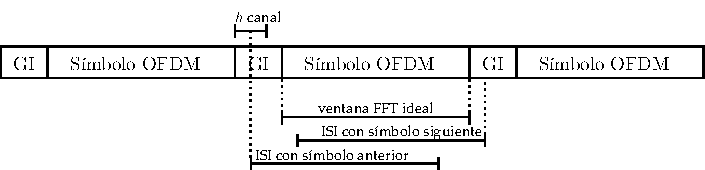
\includegraphics[width=\imsizeL ]{ventana-fft.pdf}
    \caption{Diagrama temporal de aplicación de ventana FFT a una secuencia de símbolos OFDM recibidos, describiendo la ventana ideal y los casos en los que una desviación temporal produce interferencia entre símbolos.\label{fig:ventana-fft}}  
\end{figure}

Sabiendo la duración de un símbolo OFDM y suponiendo que el reloj del receptor está suficientemente sincronizado con el reloj del transmisor, se espera que la ventana FFT esté correctamente sincronizada si se determina precisamente la muestra en la que inicia la trama recibida, por lo que identificar esta muestra es el paso inicial para evitar desvíos en temporización de símbolo.

\subsection{Desvío de frecuencia de portadora}
\label{Ss:ch3-sincronismo-frecuencia}

En los sistemas de comunicaciones digitales la señal digital equivalente en banda base que contiene la información a transmitir, $x[n]$. Al resultado de convertir la señal digital al dominio analógico se le conoce como envolvente compleja, $x(t)$, y suele representarse a través de sus componentes en fase, $x_I(t)$, y en cuadratura, $x_Q(t)$, por medio de la relación
\begin{equation}
    x(t) = x_I(t)+jx_Q(t),
\end{equation}
mientras que la señal elevada a radiofrecuencia que se transmite por el canal inalámbrico recibe el nombre de $x_R(t)$, y tiene las siguientes componentes
\begin{equation}
    x_R(t) = x_I(t)\cos(2\pi f_c t) + x_Q(t)\sin(2\pi f_c t),
\end{equation}
en donde $f_C$ es la frecuencia de portadora.

El receptor demodula $x_R(t)$ con con un demodulador coherente tal como el que se observa en la Figura \ref{fig:demod-err}, el cual utiliza osciladores locales. En una transmisión ideal el oscilador local conoce $f_C$, lo cual permite recuperar exactamente $x[n]$, siendo $x[n]=x(nT_s)$ la digitalización de la envolvente compleja a un intervalo de muestreo $T_s$. Sin embargo, oscilador local del demodulador coherente que utiliza el receptor tiene una frecuencia propia la cual se puede expresar como $f_c+\Delta f$, donde $\Delta f$ denota un error de frecuencia entre los osciladores locales del transmisor y del receptor. Al demodular la señal en estas condiciones, la señal digital recibida se verá afectada por este error, resultando en una rotación lineal en fase dada por
\begin{equation}
    y[n] = x[n] e^{j2\pi\Delta f T_s n}.
\end{equation}

\begin{figure}[t]
    \centering{}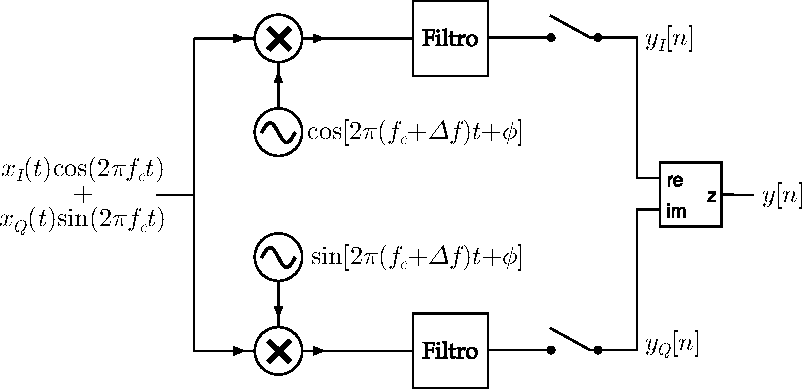
\includegraphics[width=\imsize]{demod-err.pdf}
    \caption{Esquema de demodulador coherente, considerando un error de frecuencia entre la señal entrante y el oscilador local del demodulador.\label{fig:demod-err}}  
\end{figure}

Además, si se contempla que la fase inicial de la señal es desconocida, este error en fase también se manifiesta la señal en banda base de la siguiente forma:
\begin{equation}
    y[n] = x[n] e^{j(2\pi\Delta f T_s n+\phi)}.
\end{equation}
Los algoritmos de sincronismo utilizados en este proyecto son capaces de estimar el desvío en frecuencia de portadora sin ser afectados por el error en fase.


\section{Algoritmos de sincronismo}

En esta sección se describirán dos algoritmos de sincronismo capaces de identificar la muestra inicial de la trama y el desvío de frecuencia de portadora en base al conocimiento de la secuencia de entrenamiento de símbolos cortos. Sus principios de funcionamiento son similares, en su descripción las muestras de la secuencia de entrenamiento de símbolos cortos se agrupan en un vector denotado $\mathbf{s}$, siendo conocida su longitud en muestras, $N$. 

Los métodos definen un estadístico $\Phi$ a partir de las $N$ muestras más recientes de una señal recibida, agrupadas en un vector denominado $\mathbf{y}$. Teniendo $\Phi$ se estimará un instante $\widehat{n}$, que corresponde la muestra en la que se terminó de recibir la secuencia de entrenamiento de símbolos cortos y determina el inicio de la trama. Asociado a esa muestra se obtiene una estimación del desvío de frecuencia de portadora, $\widehat{\Delta f}$. 

\subsection{Banco de correladores}
\label{S:ch3-banco}

Este método se basa en en buscar la forma conocida de la secuencia de entrenamiento de símbolos cortos en la señal recibida, calculando la correlación de $\mathbf{y}$ con señales llamadas referencias construídas a partir de $\mathbf{s}$. 

\subsubsection{Estimación de inicio de trama con una única referencia}

Se desea identificar el instante de inicio de trama, bajo la suposición de que no existe desvío en frecuencia de portadoras. En estas conciciones la función que cumple el objetivo de ser máxima en el instante de interés es simplemente el módulo de la correlación con la secuencia de entrenamiento de símbolos cortos, dada por
\begin{equation}\label{eq:correladores-1}
    \Phi_{BC}[n] = \left\lvert \sum_{k=0}^{N-1}y^\ast[n-k]s[N-k] \right\rvert.
\end{equation}

La aplicación del módulo causa que el error en fase no afecte al estadístico, ya que este es una constante compleja de módulo unitario que sale como factor común de la correlación. Para validar este desempeño, en la Figura \ref{fig:banco-xcorr1} se grafica el resultado de calcular $\Phi_{BC}$ sobre una señal compuesta únicamente por un preámbulo al cual se le ha aplicado un error en fase. se observa que $\Phi_{BC}$ alcanza su valor máximo en la muestra final de la secuencia de entrenamiento de símbolos cortos, por lo tanto $\widehat{n}$ es simplemente la muestra que lo maximiza,
\begin{equation}
    \widehat{n}_{BC} = \argmax_n\Phi_{BC}[n].
\end{equation}

\begin{figure}[t]
    \centering{}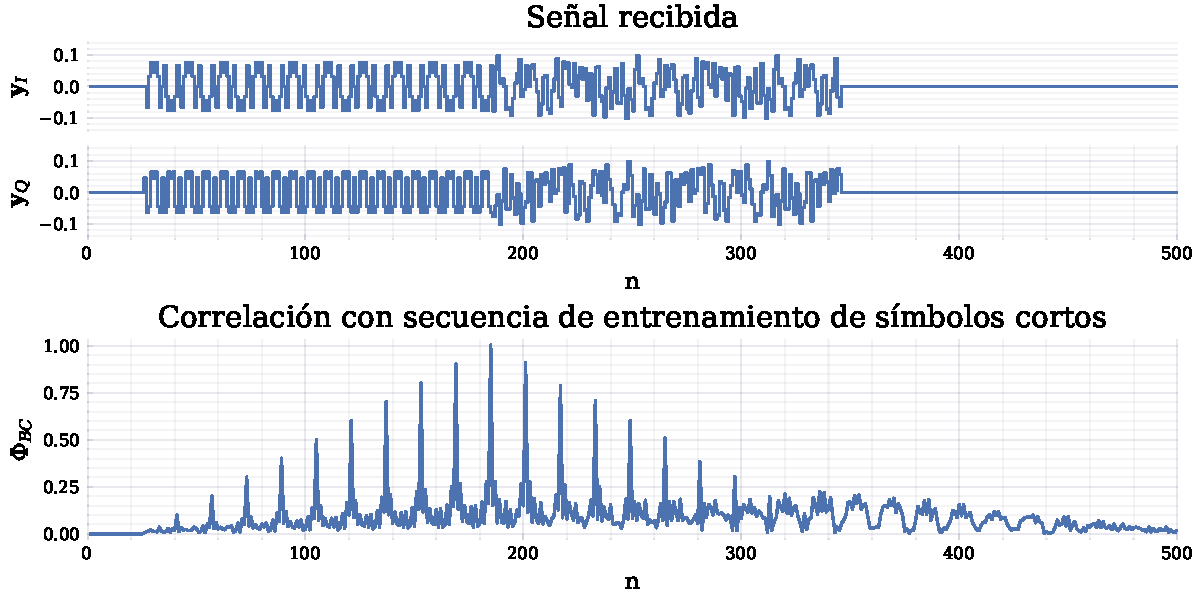
\includegraphics[width=\imsizeL]{banco-xcorr1.pdf}
    \caption{Resultado de aplicación del estadístico $\Phi_{BC}$ a una señal recibida que consiste en un preámbulo con error en fase.\label{fig:banco-xcorr1}}  
\end{figure}

\subsubsection{Estimación de desvío de frecuencia de portadora}
\label{Ss:ch3-banco-frecuencias}
El método tal como fue definido es capaz de estimar el inicio de trama, pero aún no es capaz de estimar el desvío de frecuencia de portadora. Si se contempla que $\mathbf{y}$ se ve afectada por un desvío en frecuencia de portadora tal como se modela en la Ecuación 3.3, al evaluar la Ecuación 3.5 se observará una degradación en el máximo de $\Phi_{BC}$, la que depende del factor de fase $T_s\Delta f$ y que se cuantificará definiendo el factor de degradación,
\begin{equation}
    \text{Factor de degradacíon} = \frac{\Phi_{Max}(\Delta f)}{\Phi_{Max}\lvert_{\Delta f = 0}}.
\end{equation}
El factor de degradación en función del factor de rotación de fase se calcula numéricamente y se grafica en la figura \ref{fig:degradacion}.
\begin{figure}[t]
    \centering{}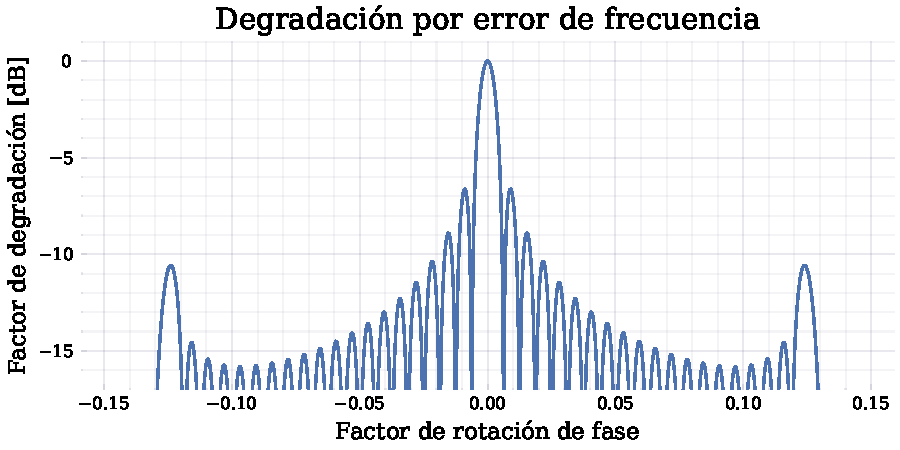
\includegraphics[width=\imsize]{degradacion-err-freq.pdf}
    \caption{Resultado del cálculo numérico del factor de degradación del estadístico $\Phi_{BC}$ en función del factor de rotación de fase.\label{fig:degradacion}}  
\end{figure}


Al tomar en cuenta que un desvío de frecuencia de portadora provoca rotación lineal en fase predecible sobre $y[n]$, el principio utilizado para la estimación con un único correlador se puede extender para estimar $\Delta f$. Se eligen $M$ frecuencias equiespaciadas dentro de un rango de frecuencias $W$ en el que se espera que se encuentre contenido $Delta f$. En particular, $M$ se elige impar, y las frecuenias equiespaciadas se denotan como $Delta f_m$, tal que
\begin{equation}
    \Delta f_m = \frac{mW}{M} \qquad\qquad m \in \left[-\frac{M-1}{2},\,\frac{M-1}{2}\right],
\end{equation}
Luego, para cada $\Delta f_m$, se genera una referencia del preámbulo con la rotación lineal en fase correspondiente a ese error en frecuencia, matemáticamente
\begin{equation}
    r_m[k] = s[k] e^{j2\pi \Delta f_m T_s k}.
\end{equation}

Una manera de determinar el paso entre frecuencias adyancentes para las múltiples referencias, consiste en valerse del factor de degradación, bajo la convención de que el mismo tome el valor de -3 dB, lo que implica que el factor de rotación de fase sea menor a 0,0037, de donde se fijan los valores para $W$ y $M$. Aplicar este criterio considerando $T_{SHORT} = 8 \mu\text{s}$ y FFT de 64 puntos se obtiene que el espaciamiento en frecuencias debe ser de 21 kHz como máximo. En la Figura \ref{fig:references} se visualizan algunas referencias generadas usando este criterio.
\begin{figure}[t]
    \centering{}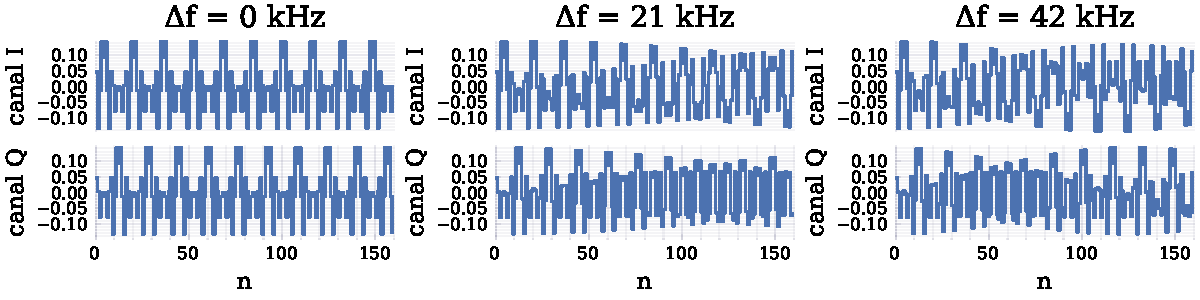
\includegraphics[width=\imsizeL]{references.pdf}
    \caption{Ejemplos de referencias generadas considerando rotación lineal en fase producto de diferentes errores de frecuencia.\label{fig:references}}  
\end{figure}


Teniendo las múltiples referencias se extiende vectorialmente el estadístico $\Phi_{BC}$ calculado
\begin{equation}\label{eq:correladores-banco}
    \overline{\Phi}_{BC}[n,m] = \left\lvert \sum_{k=1}^{N}y^\ast[n-k]r_m[N-k] \right\rvert
\end{equation}

El resultado de aplicar $\overline{\Phi}_{BC}$ a una señal con rotación lineal en fase visualiza en la figura \ref{fig:banco-xcorrN}. Se observa que los índices $n$ y $m$ que maximizan el estadístico son, respectivamente, la muestra final de la secuencia de entrenamiento de símbolos cortos y el índice de la referencia con $\Delta f_m$ más cercano a $\Delta f$. Estos índices serán $\widehat{n}_{BC}$ y $\widehat{m}_{BC}$, y este último se usará para calcular $\widehat{\Delta f}_{BC}$
\begin{equation}
    \widehat{n}_{BC}, \widehat{m}_{BC} = \argmax_{n,m}\overline{\Phi}_{BC}[n,m] \quad \implies \quad     \widehat{\Delta f}_{BC} = \frac{W}{M} \widehat{m}_{BC}
\end{equation}

\begin{figure}[t]
    \centering{}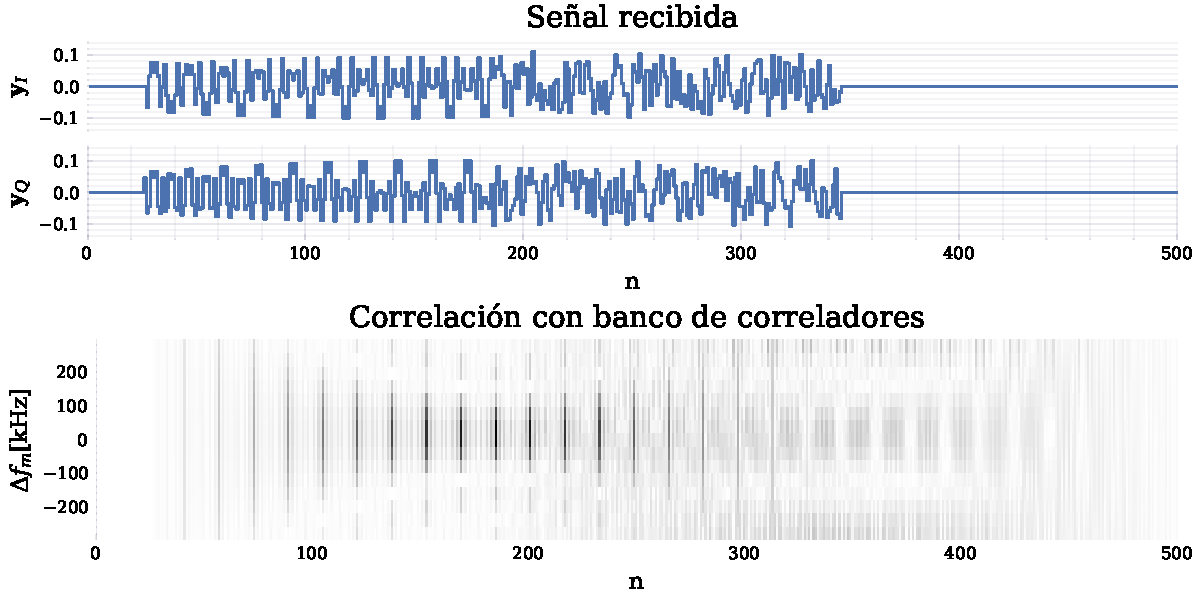
\includegraphics[width=\imsizeL]{banco-xcorrN.pdf}
    \caption{Resultado de aplicación del estadístico $\overline{\Phi}_{BC}$ a una señal recibida que consiste en un preámbulo con rotación lineal en fase provocado por un desvío de frecuencia de protadora de 21 kHz.\label{fig:banco-xcorrN}}  
\end{figure}


\subsection{Método \textit{delay and correlate}}
\label{S:ch3-dac}

El método \textit{Delay and Correlate}, a diferencia del banco de correladores, no usa la forma de onda explícita de la secuencia de entrenamiento de símbolos cortos para sincronizar, sino que utiliza el conocimiento de su periodicidad. La estrategia se centra en tomar las últimas $N$ muestras de la señal recibida y evaluar si cumplen con la periodicidad esperada de la secuencia de entrenamiento de símbolos cortos. 

\subsubsection{Sincronización en tiempo y frecuencia}
\label{Ss:ch3-dac-principio}

En su versión más simple, este método detecta la periodicidad de la señal comparando la primer mitad del intervalo de las últimas $N$ muestras recibidas con la segunda mitad del mismo, usando el factor de correlación, es decir
\begin{equation}\label{eq:dac-estimator}
    \Phi_{DC}[n] = \sum_{k=0}^{R}y^\ast[n-k]y[n-k-R],
\end{equation}

donde el parámetro $R$ es exáctamente $N/2$ donde $N$ es la longitud del preámbulo. Se puede verificar que el módulo de $\Phi_{DC}$ es máximo cuando las señales correspondientes a los dos intervalos evaluados son idénticas salvo por una rotación relativa en fase. De esta forma $\widehat{n}_{DC}$ nuevamente será la muestra que maximice el estadístico,
\begin{equation}
    \widehat{n}_{DC} = \argmax_n\lvert \Phi_{DC}[n] \lvert.
\end{equation}

A su vez, la fase de $\Phi_{DC}$ contiene información de la diferencia relativa en fase de las señales en cada intervalo, lo que permite estimar el error en frecuencia que provocó esa rotación. La fórmula para estimar el error en frecuencia con este método es la siguiente:+
\begin{equation}\label{eq:freq-est-dac}
    \widehat{\Delta f}_{DC} = \frac{1}{2\pi L T_S}\angle\Phi_{DC}[\widehat{n}_{DC}].
\end{equation}

Los resultados de la aplicación de $\Phi_{DC}$ sobre una señal recibida con rotación lineal en fase se visualizan en la figura \ref{fig:dac-result}.
\begin{figure}[t]
    \centering{}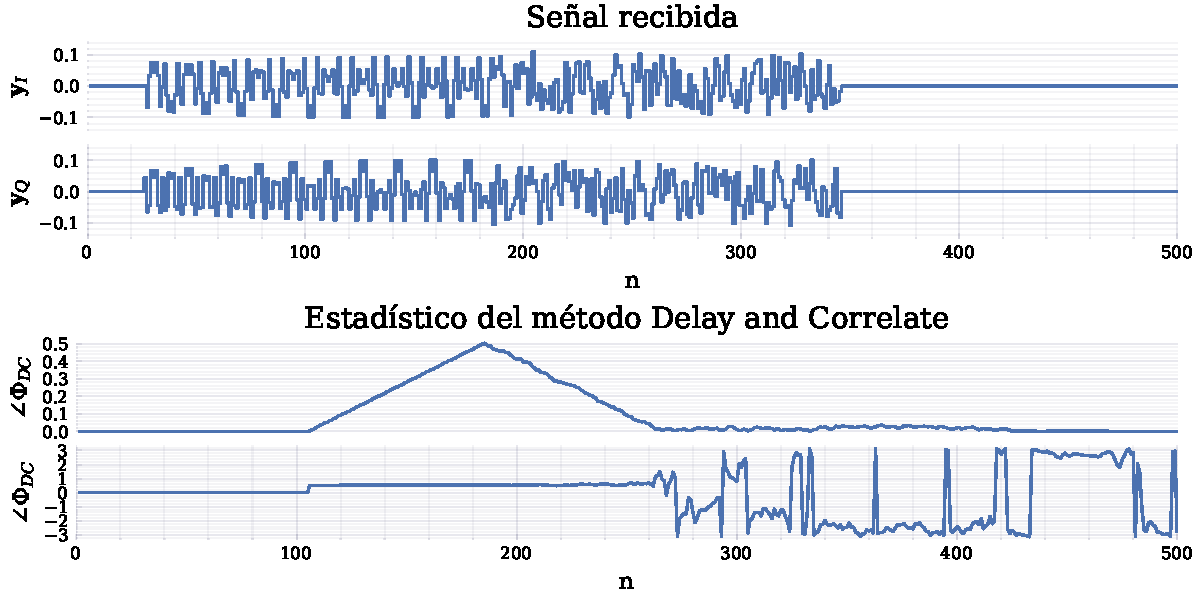
\includegraphics[width=\imsizeL]{delay-and-correlate-result.pdf}
    \caption{Resultado de aplicación del estadístico $\Phi_{DC}$ a una señal recibida que consiste en un preámbulo con error de frecuencia.\label{fig:dac-result}}  
\end{figure}


\subsection{Implementaciones en LabVIEW}
\label{Ss:ch3-labview}

La implementación en LabVIEW de los métodos instancia algoritmos para calcular los estadísticos de sincronismo en determinado instante de muestreo $n$. En estos casos se considera una ventana de evaluación que recibe el nombre de $\mathbf{v}$, y son las últimas $N$ muestras recibidas,
\begin{equation}
    \mathbf{v}[n] = 
    \begin{bmatrix}
        y[N-n+1] &  \cdots & y[n]
    \end{bmatrix}.
\end{equation}
En las expresiones para calcular los estadísticos usando cada método, $\overline{\Phi}_{BC}$ y $\Phi_{DC}$ respectivamente, se omite el índice $n$ ya que este es implícitamente el instante de muestreo en el que se ejecutan las operaciones. 


\subsubsection{Implementación del banco de correladores}

\begin{figure}[t]
    \centering{}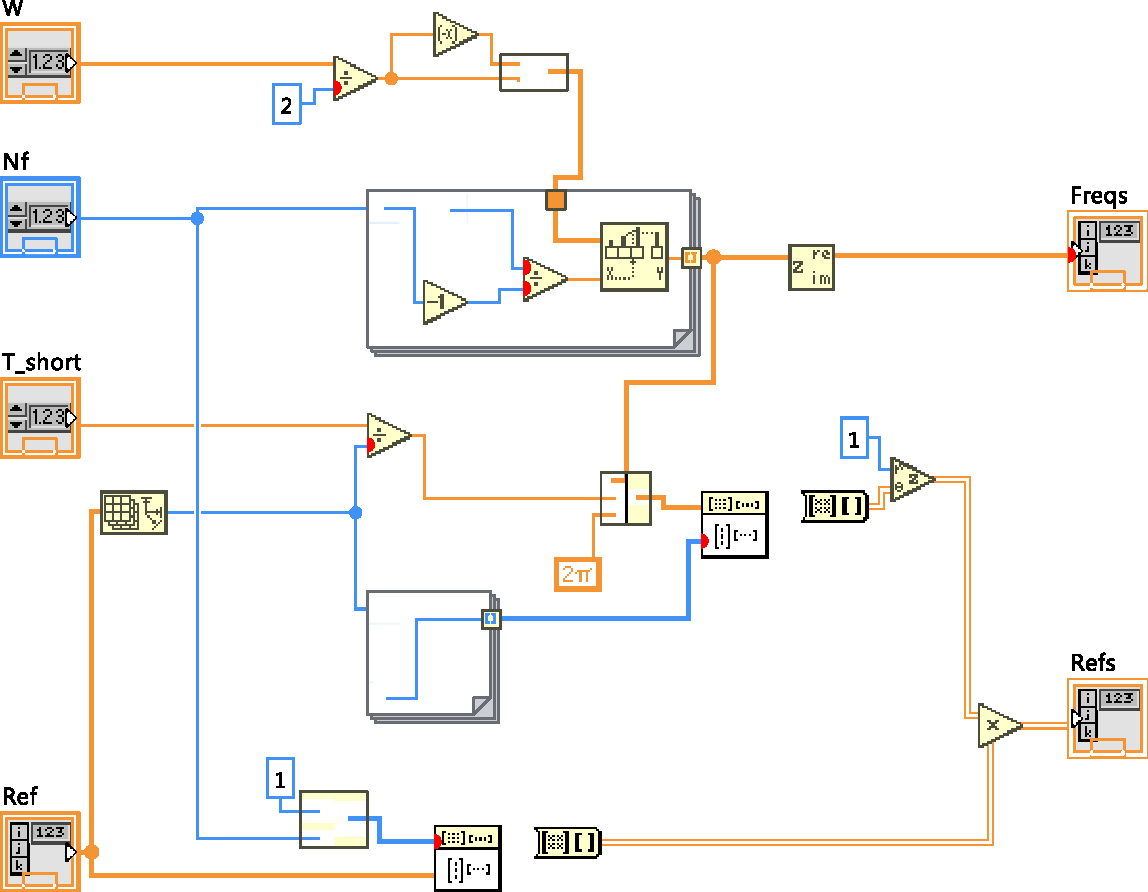
\includegraphics[width=\imsizeL]{xpstopdf/refs.pdf}
    \caption{Diagrama en bloques de las referencias necesarias para calcular el estadístico $\overline{\Phi}_{BC}$ en LabVIEW.\label{fig:refs_lv}}  
\end{figure}

\begin{figure}[t]
    \centering{}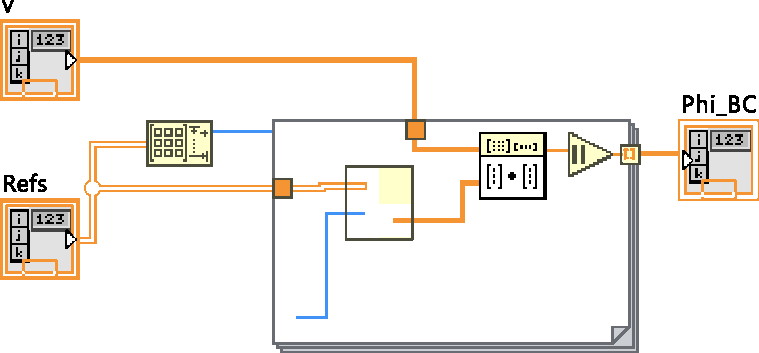
\includegraphics[width=\imsize]{xpstopdf/bancox.pdf}
    \caption{Diagrama de bloques del cálculo del estadístico $\overline{\Phi}_{BC}$ en LabVIEW.\label{fig:bancox_lv}}  
\end{figure}

El cálculo del estadístico $\overline{\Phi}_{BC}$ implementado en LabVIEW se ve en el diagrama de bloques presentado en la Figura \ref{fig:bancox_lv}. Requiere de matriz de referencias, llamada $R$, la cual es una matriz de $M \times N$ en donde la fila $m$ son las $N$ muestras de la secuencia de entrenamiento de símbolos cortos con el correspondiente error de frecuencia aplicado,
\begin{equation}
    R_{M\times N} = \begin{bmatrix}
       \cdots & \mathbf{r}_{0} & \cdots\\
       \cdots & \mathbf{r}_{1} & \cdots\\
       & \vdots & \\
       \cdots & \mathbf{r}_{M-1} & \cdots
    \end{bmatrix}.
\end{equation}
Ésta se construye a partir del diagrama de bloques presentado en la Figura \ref{fig:refs_lv}, en el que se toma un rango de errores de frecuencia $W$ y un número de frecuencias $M$, la secuencia de entrenamiento de símbolos cortos $s$ y su duración $T_{SHORT}$. Este diagrama en bloques retorna la matriz de referencias y un vector de errores de frecuencia correspondiente a cada fila de la matriz.

El diagrama de bloques presentado en la Figura \ref{fig:bancox_lv} calcula $\overline{\Phi}_{BC}$ a partir de $R$ y $\mathbf{v}$. Para hacerlo itera sobre las filas de $R$, en cada iteración calculando el factor de correlación de la ventana con la referencia. Esto se consigue con la operación producto interno, y el resultado es un vector de $M$ elementos
\begin{equation}
    \overline{\Phi}_{BC} = \begin{bmatrix}
        \mathbf{v} \cdot \mathbf{r}_{0}\\
        \mathbf{v} \cdot \mathbf{r}_{1}\\
        \vdots\\
        \mathbf{v} \cdot \mathbf{r}_{M-1}
    \end{bmatrix}.
\end{equation}

\subsubsection{Implementación del método \textit{delay and correlate}}

La implementación del método delay and correlate en LabVIEW resulta mucho más simple, su diagrama en bloques se presenta en la Figura \ref{fig:delayx_lv}. El método calcula $L = N/2$ y usa ese valor para particionar $\mathbf{v}$, luego calcula el factor de correlación entre las dos partes por medio del producto interno,
\begin{equation}\textstyle
    \Phi_{DC} = \mathbf{v}_1 \cdot \mathbf{v}_2,
\end{equation}
donde $\mathbf{v}_1$ y $\mathbf{v}_2$ son la primera y la segunda mitad de $\mathbf{v}$ respectivamente.

\begin{figure}[t]
    \centering{}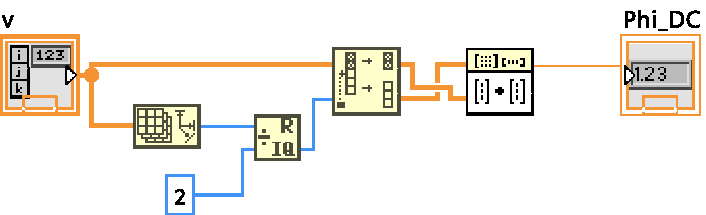
\includegraphics[width=\imsize]{xpstopdf/delayx.pdf}
    \caption{Diagrama de bloques del cálculo del estadístico $\Phi_{DC}$ en LabVIEW.\label{fig:delayx_lv}}  
\end{figure}


\section{Resumen del capítulo}

En este capítulo se definieron los tipos de de error de sincronismo que se deben estimar para la correcta recepción de tramas OFDM: el desvío de temporización de símbolo y el desvío de frecuencia de portadora. 

Se definieron dos métodos que son capaces de realizar un sincronismo inicial tanto en tiempo como en frecuencia, haciendo uso del conocimiento del preámbulo definido en el estándar IEEE 802.11, estos métodos son el banco de correladores y el método de retardo y correlación. Una vez descritos los métodos se ilustró cómo fueron implementados en LabVIEW por medio de diagramas en bloques. 

%%% Local Variables: 
%%% mode: latex
%%% TeX-master: "template"
%%% End: 
